\graphicspath{{./images/algo}}
\section{Аналитическая часть}

\subsection{Экспортирование результата в таблицу}

Для нахождения оптимального расположения датчика, будем перебирать интересующие точки, и температуру в них запишем в таблицу для дальнейшего сравнения. Самым простым вариантом будет рассмотреть сетку из точек $9 \times 9 \times 9$ (Рис. \ref{9x9x9}).

\begin{figure}[H]
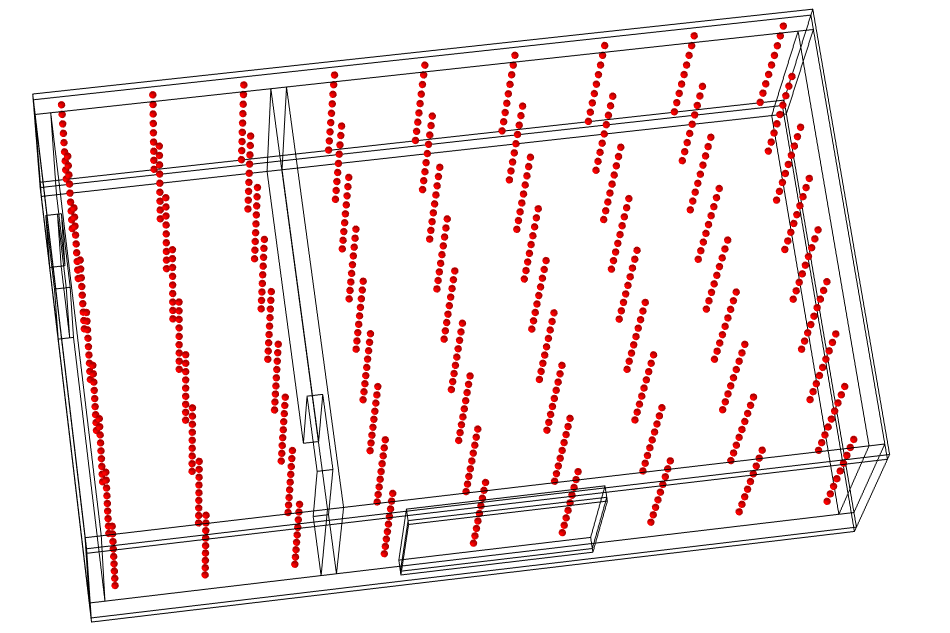
\includegraphics[width=\textwidth]{comsol/interesting_points_9x9x9.png}
\caption{}
\label{9x9x9}
\end{figure}

Однако, можно заметить, что большинство точек находятся не у стены, а значит и установить датчик в них будет проблематично. Поэтому более оптимальным вариантом будет рассмотреть сетку вдоль каждой из стен, пола и потолка (Рис. \ref{interesting_points}). Точки будем распологать на некотором расстоянии от стены ($15$ см), так как температура воздуха может достаточно сильно отличаться от температуры стены.

\begin{figure}[H]
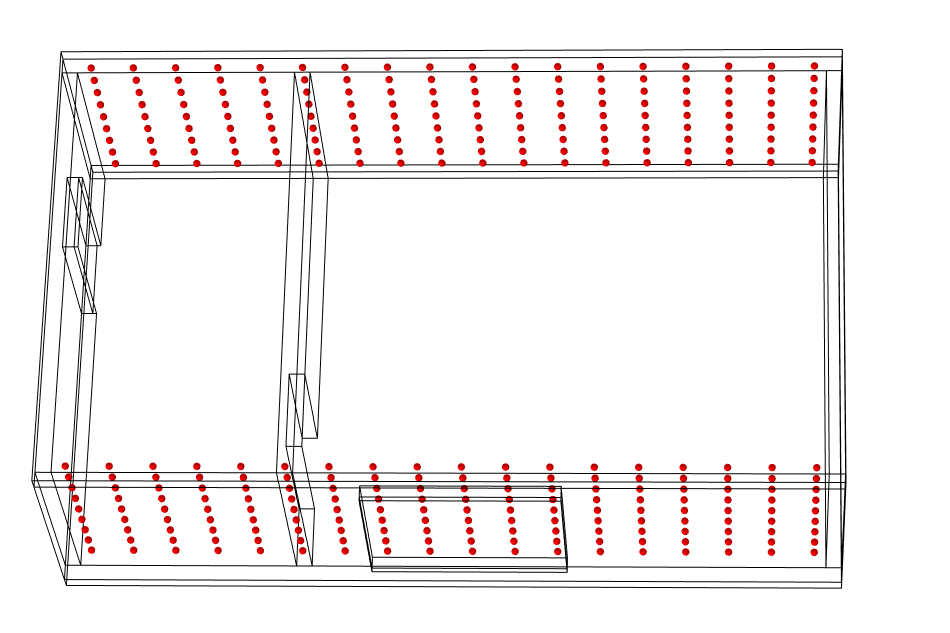
\includegraphics[width=0.5\textwidth]{comsol/interesting_points_X.png}
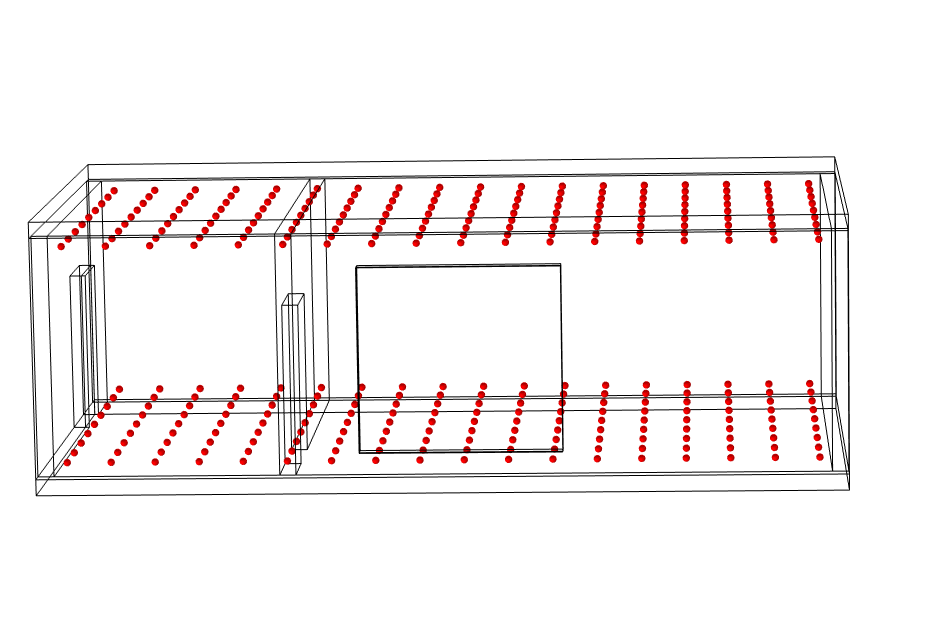
\includegraphics[width=0.5\textwidth]{comsol/interesting_points_Z.png}
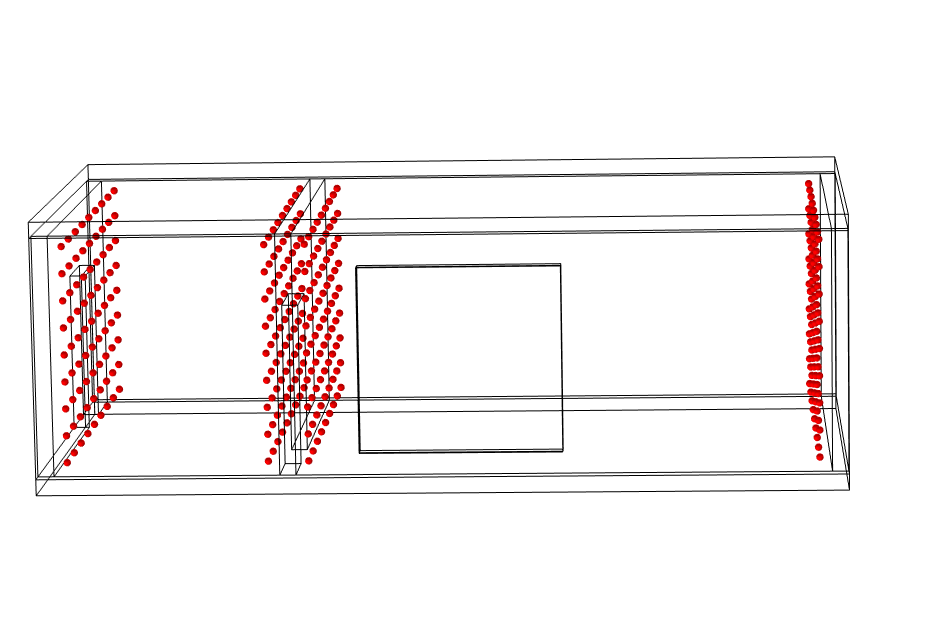
\includegraphics[width=\textwidth]{comsol/interesting_points_Y.png}
\caption{}
\label{interesting_points}
\end{figure}

Полученная таблица температур выглядит так:

\begin{table}[H]
\centering
\begin{tabular}{c|c|c|c|c|c}
\textbf{Time (s)} & \textbf{Point 1} & \textbf{Point 2} & ... & \textbf{Point N} & \textbf{Ambient} \\ \hline
0                 & 20.0             & 19.4             &     & 20.8              & 17.9             \\
300               & 19.9             & 19.4             &     & 20.7              & 17.9             \\
600               & 19.9             & 19.4             &     & 20.6              & 17.9             \\
...               &                  &                  &     &                   &                  \\
345600            & 21.2             & 21.5             &     & 20.8              & 19.9            
\end{tabular}
\end{table}

\newpage


\subsection{Критерий оптимальности точки}
\label{algo-2}

Теперь надо определить критерий оптимальности точки. Между внутренней температурой помещения и внешней температурой есть явная линейная зависимость \cite{pashchenko-rassadin}. Однако, для нахождения наиболее точной регрессии, надо определить временной сдвиг температур. Из физической сущности процесса тепломассообмена следует, что нагрев и охлаждение помещения под воздействием наружной температуры происходит не мгновенно, а с некоторым временным сдвигом. Например, на графике (Рис. \ref{indent1}) изображено изменение внешней температуры (синяя кривая) и температура в одной из внутренних точек (оранжевая кривая). Можно видеть, что точки перелома у синей кривой встречаются раньше, чем у оранжевой.

\begin{figure}[H]
\centering
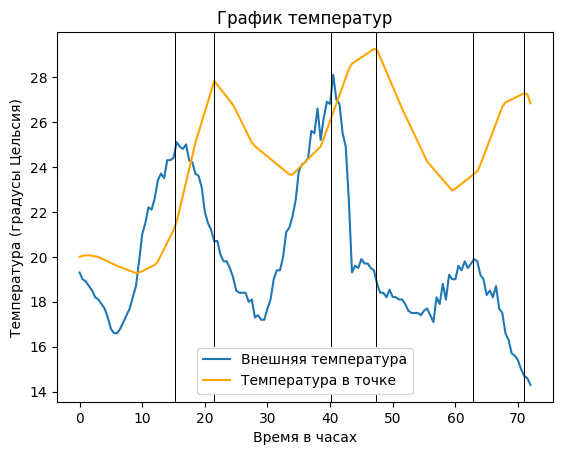
\includegraphics[width=0.9\textwidth]{graphics/indent.png}
\caption{}
\label{indent1}
\end{figure}

\newpage

Величину этого сдвига будем определять, сдвигая последовательно массив значений наружной температуры относительно массива внутренней температуры на шаг $t$ и вычисляя значение линейной корреляции Пирсона \cite{pearson} между полученными рядами. В нашем случае шаг $t$ равен шагу в модели и составляет $5$ минут. На полученном графике (Рис. \ref{indent2}) видно, что после сдвига точки экстремума гораздо лучше накладываются друг на друга, что в свою очередь улучшает точность линейной регрессии. Сдвиг при этом для каждой точки может быть разный.

\begin{figure}[H]
\centering
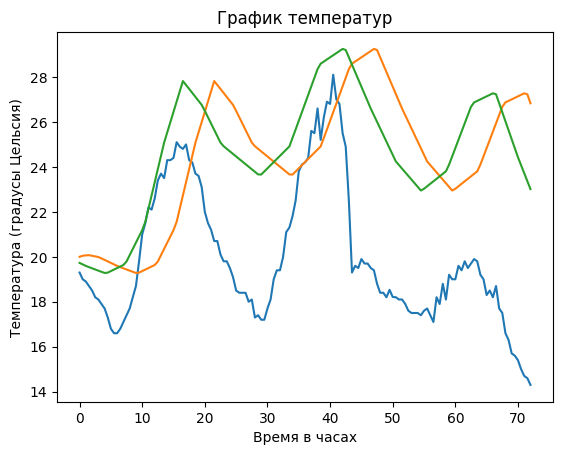
\includegraphics[width=0.9\textwidth]{graphics/indent_2.png}
\caption{}
\label{indent2}
\end{figure}

\newpage 


\subsection{Описание алгоритма}

Теперь, когда определили временной сдвиг, можем строить линейную регрессию. Для этого у нас есть 2 датасета: тренировочный, в котором записаны посчитанные температуры за 4 дня с 04.08.2020 по 07.08.2020, и тестовый, в котором температуры за 3 дня с 09.08.2020 по 11.08.2020. Мы перебираем все возможные столбцы температур из тренировочной таблицы, для каждой находим свой сдвиг, при котором коэффициент линейной корреляции Пирсона со столбцом внешних температур максимален. Затем считаем коэффициенты линейной регрессии сдвинутого столбца. Далее, используя полученные коэффициенты и сдвиг, аппроксимируем температуру воздуха снаружи из тестового датасета. Для полученной аппроксимации считаем коэффициент детерминации $R^2$. Точка с наибольшим коэффициентом считается оптимальной.

Стоит отметить, что в нашем алгоритме мы по внутренней температуре предсказываем внешнюю. Хотя логично было бы наоборот, по температуре снаружи предсказывать температуру внутри. Однако, это взаимно обратные задачи, и линейная регрессия легко пересчитывается. Поэтому на результат это не будет влиять. И при этом будет удобней сравнивать точки, а именно рисовать графики.

\newpage

\subsection{Результаты}

На графике ниже (Рис. \ref{result}) показан результат работы алгоритма. 

\begin{figure}[H]
\centering
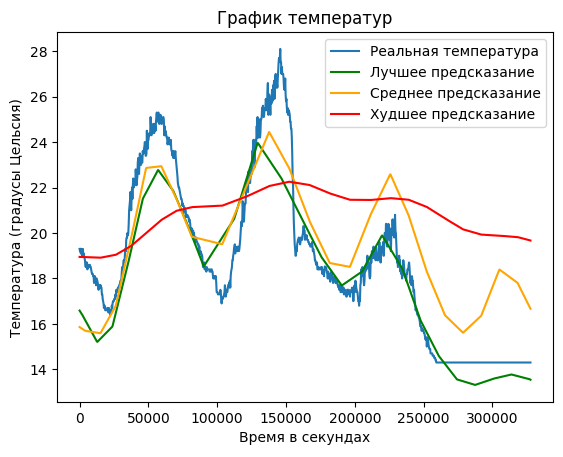
\includegraphics[width=0.9\textwidth]{graphics/result.png}
\caption{}
\label{result}
\end{figure}

Можно видеть, что в точках локальных минимумов и максимумов разница предсказаний доходит до градуса между лучшим и средним. Худшее же предсказание показывает наименьшее колебание температур. Точка с худшим предсказанием находится в самом центре комнаты (Рис. \ref{interesting-points-result}, для наглядности сократим количество интересующих расположений до $3 \times 3 \times 3$). Это логичный результат, так как все остальные точки находятся рядом со стенами, которые напрямую взаимодействуют с окружающей средой, и поэтому температура в них также сильнее зависит от внешней температуры. Лучшее расположение датчика оказывается рядом со стеклом, что тоже логично, так как на стены светит солнце и излишне нагревает их. Окно в свою очередь не подвержено солнечной радиации, поэтому и температура будет зависеть в основном от внешней. Для остальных точек сложнее делать выводы, так как например точки над окном находятся на юге, а значит и греются больше всего. Тем не менее, предсказания в них являются лучшими после точки у окна.

Также нужно учитывать саму модель. Данное помещение смоделировано как отдельное здание, а не как одна комната в большом доме. То есть все стены и потолок взаимодействуют со внешней средой, на них светит солнце. Для комнаты было бы так, что температура внутренних стен была бы более стабильной, а значит и результаты предсказаний были бы другими.


\begin{figure}[H]
\centering
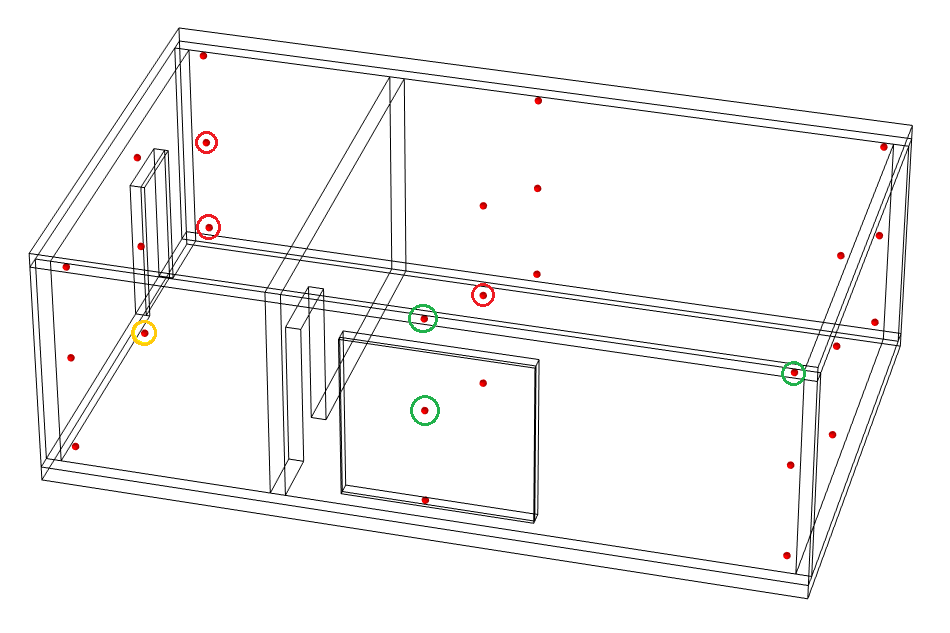
\includegraphics[width=0.9\textwidth]{interesting_points_result.png}
\caption{}
\label{interesting-points-result}
\end{figure}








































